% DYSLEXIA SWITCH
\newif\ifdys
		
				% ENABLE or DISABLE font change
				% use XeLaTeX if true
				\dystrue
				\dysfalse


\ifdys

\documentclass[a4paper, 14pt]{extarticle}
\usepackage{amsmath,amsfonts,amsthm,amssymb,mathtools}

\tracinglostchars=3 % Report an error if a font does not have a symbol.
\usepackage{fontspec}
\usepackage{unicode-math}
\defaultfontfeatures{ Ligatures=TeX,
                      Scale=MatchUppercase }

\setmainfont{OpenDyslexic}[Scale=1.0]
\setmathfont{Fira Math} % Or maybe try KPMath-Sans?
\setmathfont{OpenDyslexic Italic}[range=it/{Latin,latin}]
\setmathfont{OpenDyslexic}[range=up/{Latin,latin,num}]

\else

\documentclass[a4paper, 12pt]{extarticle}

\usepackage[utf8x]{inputenc}
\usepackage{lmodern,textcomp}
\usepackage{amsmath,amsfonts,amsthm,amssymb,mathtools}

\fi


\usepackage[french]{babel}
\usepackage[
a4paper,
margin=2cm,
nomarginpar,% We don't want any margin paragraphs
]{geometry}
\usepackage{icomma}

\usepackage{fancyhdr}
\usepackage{array}

\usepackage{multicol, enumerate}
\newcolumntype{P}[1]{>{\centering\arraybackslash}p{#1}}


\usepackage{stackengine}
\newcommand\xrowht[2][0]{\addstackgap[.5\dimexpr#2\relax]{\vphantom{#1}}}

% theorems

\theoremstyle{plain}
\newtheorem{theorem}{Th\'eor\`eme}
\newtheorem*{theorem*}{Th\'eor\`eme}
\newtheorem*{sol}{Solution}
\theoremstyle{definition}
\newtheorem{ex}{Exercice}

% corps
\newcommand{\C}{\mathcal{C}}
\newcommand{\R}{\mathbb{R}}
\newcommand{\Rnn}{\mathbb{R}^{2n}}
\newcommand{\Z}{\mathbb{Z}}
\newcommand{\N}{\mathbb{N}}
\newcommand{\Q}{\mathbb{Q}}

% domain
\newcommand{\D}{\mathcal{D}}


% date
\usepackage{advdate}
\AdvanceDate[0]


% plots
\usepackage{pgfplots}

% for calligraphic C
\usepackage{calrsfs}

% SOLUTION SWITCH
\newif\ifsolutions
				\solutionstrue
				\solutionsfalse

\ifsolutions
	\newcommand{\exe}[2]{
		\begin{ex} #1  \end{ex}
		\begin{sol} #2 \end{sol}
	}
\else
	\newcommand{\exe}[2]{
		\begin{ex} #1  \end{ex}
	}
	
\fi

\begin{document}
\pagestyle{fancy}
\fancyhead[L]{Seconde 13}
\fancyhead[C]{\textbf{Calcul de hauteur, d'aire, de volume \ifsolutions -- Solutions  \fi}}
\fancyhead[R]{\today}


\exe{
	\begin{multicols}{2}
	Considérons le triangle $ABC$ d'aire $\text{Aire}(ABC) = \dfrac{3}{10}$ et tel que $AB=\dfrac34$ et $CD =\dfrac25$.
	
	Est-ce que les droites $(AB)$ et $(CD)$ sont perpendiculaires ?
	
	\begin{center}
	\begin{tikzpicture}[scale=.6]
		\draw[-, thick, black] (0,0) node{$\bullet$} -- (4, 3) node{$\bullet$};
		\draw[-, thick, black] (4, 3) node{$\bullet$} -- (1,4) node{$\bullet$};
		\draw[-, thick, black] (1,4) node{$\bullet$} -- (0,0) node{$\bullet$};
		
		\node[black, below] at  (0,0)  {$A$};
		\node[black, right] at  (4, 3)  {$B$};
		\node[black, above] at  (1,4) {$C$};
		
		
		\node[black] at  (2.5,2.5*3/4) {$\bullet$};
		\node[black, below] at  (2.5,2.5*3/4) {$D$};
	
	\end{tikzpicture}
	\end{center}
	
	\end{multicols}
}{}


\exe{
	Considérons le triangle $ABC$ comme à l'exercice 1 et d'aire $\text{Aire}(ABC) = 8$ et tel que $AB=4$ et $AC =5$.
	
	
	Quelle longueur $AD$ doit-on choisir pour que les droites $(AB)$ et $(DC)$ soient perpendiculaires ?
}{}

\exe{[10, 11 page 140] \, \vspace{-15pt}
	\begin{center}
	\begin{multicols}{2}
	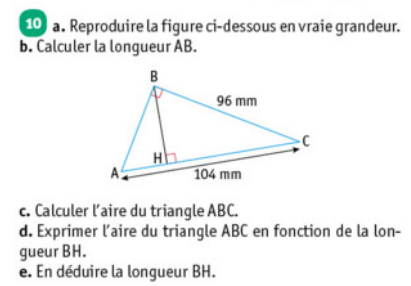
\includegraphics[scale=.6]{10p140.png}
	
	\, \,
	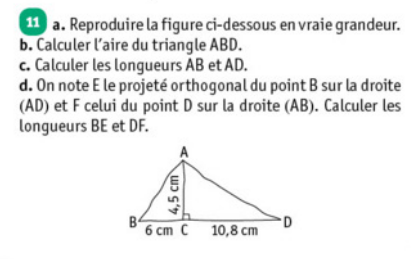
\includegraphics[scale=.55]{11p140.png}
	\end{multicols}
	\end{center}
}
{}

\exe{[53, 57 page 147] \, \vspace{-15pt}
	\begin{center}
	\begin{multicols}{2}
	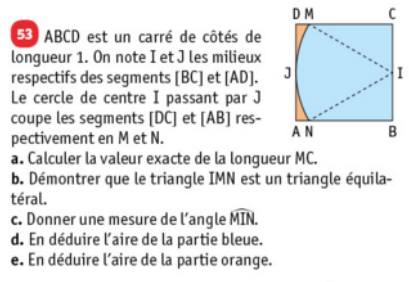
\includegraphics[scale=.6]{53p147.png}
	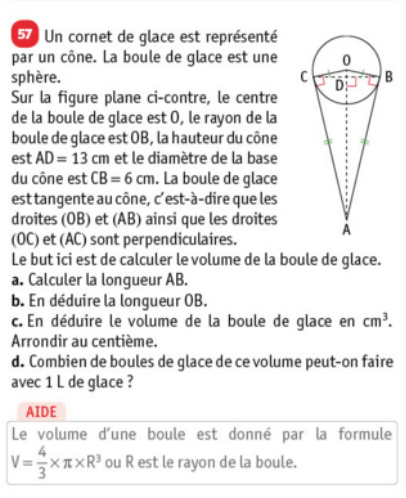
\includegraphics[scale=.55]{57p147.png}
	\end{multicols}
	\end{center}
}{}

\end{document}
